\chapter{Performance}
 \label{chap:perf}
 
 The major goal of this work is to have a fully automated model generation in \emph{PyNEST} without drastically degrading the performance of the simulation script and encouraging users to use the new implemented \emph{JIT} module. In order to test the impact of the using \emph{JIT} in the simulation script, we need to test different configurations that might eventually appear when running the simulation with \emph{JIT}. Firstly, we test the neuronal network with the script explicitly calling \emph{PyNESTML} module and the \texttt{nest.Install} function and  consider its running time as our base model. Secondly, we run the same neuronal network, but this time everything is controlled by the \emph{JIT} module. Thirdly, we repeat the same experiment, but this time we choose a neuronal network that includes using a custom implemented synapse.
 
 As the \emph{NestKernel} does not completely utilize the new data structure behind \emph{vectorization}, we can not really make meaningful evaluation of its impact on the performance. Therefore, we only decided to compare single functions between simple and \emph{vectorized} models. Such functions are \texttt{nest.Create} and \texttt{nest.GetStatus}.
 
 From the \emph{JIT} perspective, we do not really care about the size of the network or its behave, because we only simply retrieve the model and make it available to the simulation script. In that case, any neuronal network should be fine to test with. In the first experiment, we choose a random balanced network as  described by \emph{Brunel} \citep{brunel2000dynamics}. For the second experiment with synapse, we build a network with a spike-timing dependent plasticity (STDP) synaptic type.
 
 
 For \emph{vectorization}, we only test the \texttt{nest.Create} and \texttt{nest.GetStatus} functions by creating instances of the \emph{Izhikevich} \citep{1257420} with modifying the number of instances and the number of used threads.
 
\section{The JIT Module}

\subsection*{Running The JIT Module Without An external Synapse Type}

In the first experiment in testing the \emph{JIT} module, we run the \emph{Brunel} network by explicitly using the \emph{PyNESTML} to generate the code for the required model, and then we run the same network by using the \emph{JIT} module. The result of the experiment can be found in the \autoref{fig:max_average_min}.

\begin{figure}[ht!]
    \centering
    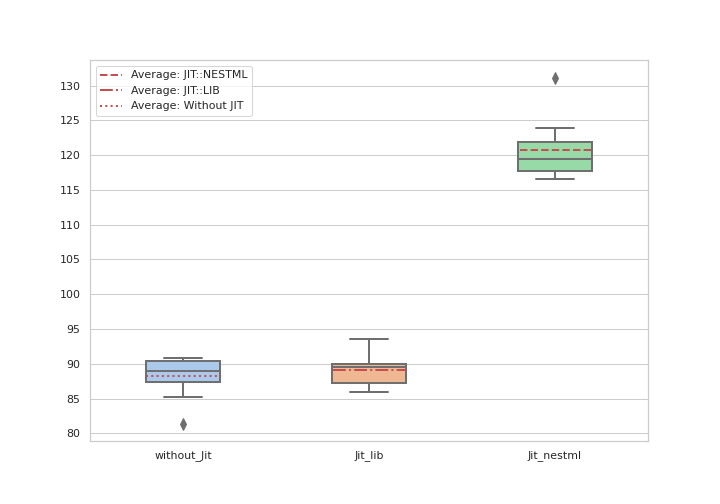
\includegraphics[width=\textwidth]{src/pic/box_plot_three.png}
    \caption{The max-average-min runtime in seconds}
    \label{fig:max_average_min}
\end{figure}

In the \autoref{fig:max_average_min}, we show the runtime of three possible cases. The first is when we are explicitly calling the \emph{PyNESTML} module, and it is labeled with \emph{Without\_Jit}. The second case is when running the simulation with an external model using the \emph{JIT} module, and it is labeled with \emph{Jit\_Nestml}. The last case is when using \emph{JIT} with an external library, and usually it is the result after generating the code for the \emph{nestml} model. The last case is labeled with \emph{Jit\_Lib} in the plot. In each of the three cases, we show the \emph{maximum}, \emph{average} and \emph{minimum} required to run the simulation.

The first case (i.e., \emph{Without\_Jit}) has the lowest runtime, and it took on average 90 seconds to finish the simulation. In the other hand, the average runtime for the \emph{Jit\_Nestml} took around 130 seconds, and the \emph{Jit\_Lib} took around 90 seconds.  Both the first case and the last case have almost the same behavior, with the exception that the \emph{minimum} runtime for the last case was a bit higher. This can be explained with the introduced overhead in the \emph{JIT} module, and it is most significant in the second case. All the three values of the \emph{Jit\_Nestml} are the highest among the other cases, and it can be explained by the time required for searching the model and maintaining \texttt{NodeCollectionProxy} by converting the \texttt{JitNodeCollection} to the real \texttt{NodeCollection} instances and copying the parameters from one instance to the other.


\subsection*{Running The JIT Module with An external Synapse Type}

In the second experiment, we ran the \emph{STDP windows} simulation script from the \texttt{NESTML} tutorial, and again we compared the simulation runtime with using \emph{JIT} against the original script without \emph{JIT}. In this tutorial, we have a function that is responsible for creating the instances of the models and creating the network, and it is called multiple times in a \emph{for-loop} (exactly 151 times). In the \emph{JIT} settings, it means that the model will be searched many times, and we would expect that only the first iteration will take most of the time in comparison to the subsequent iterations. 

\begin{figure}[ht!]
    \centering
    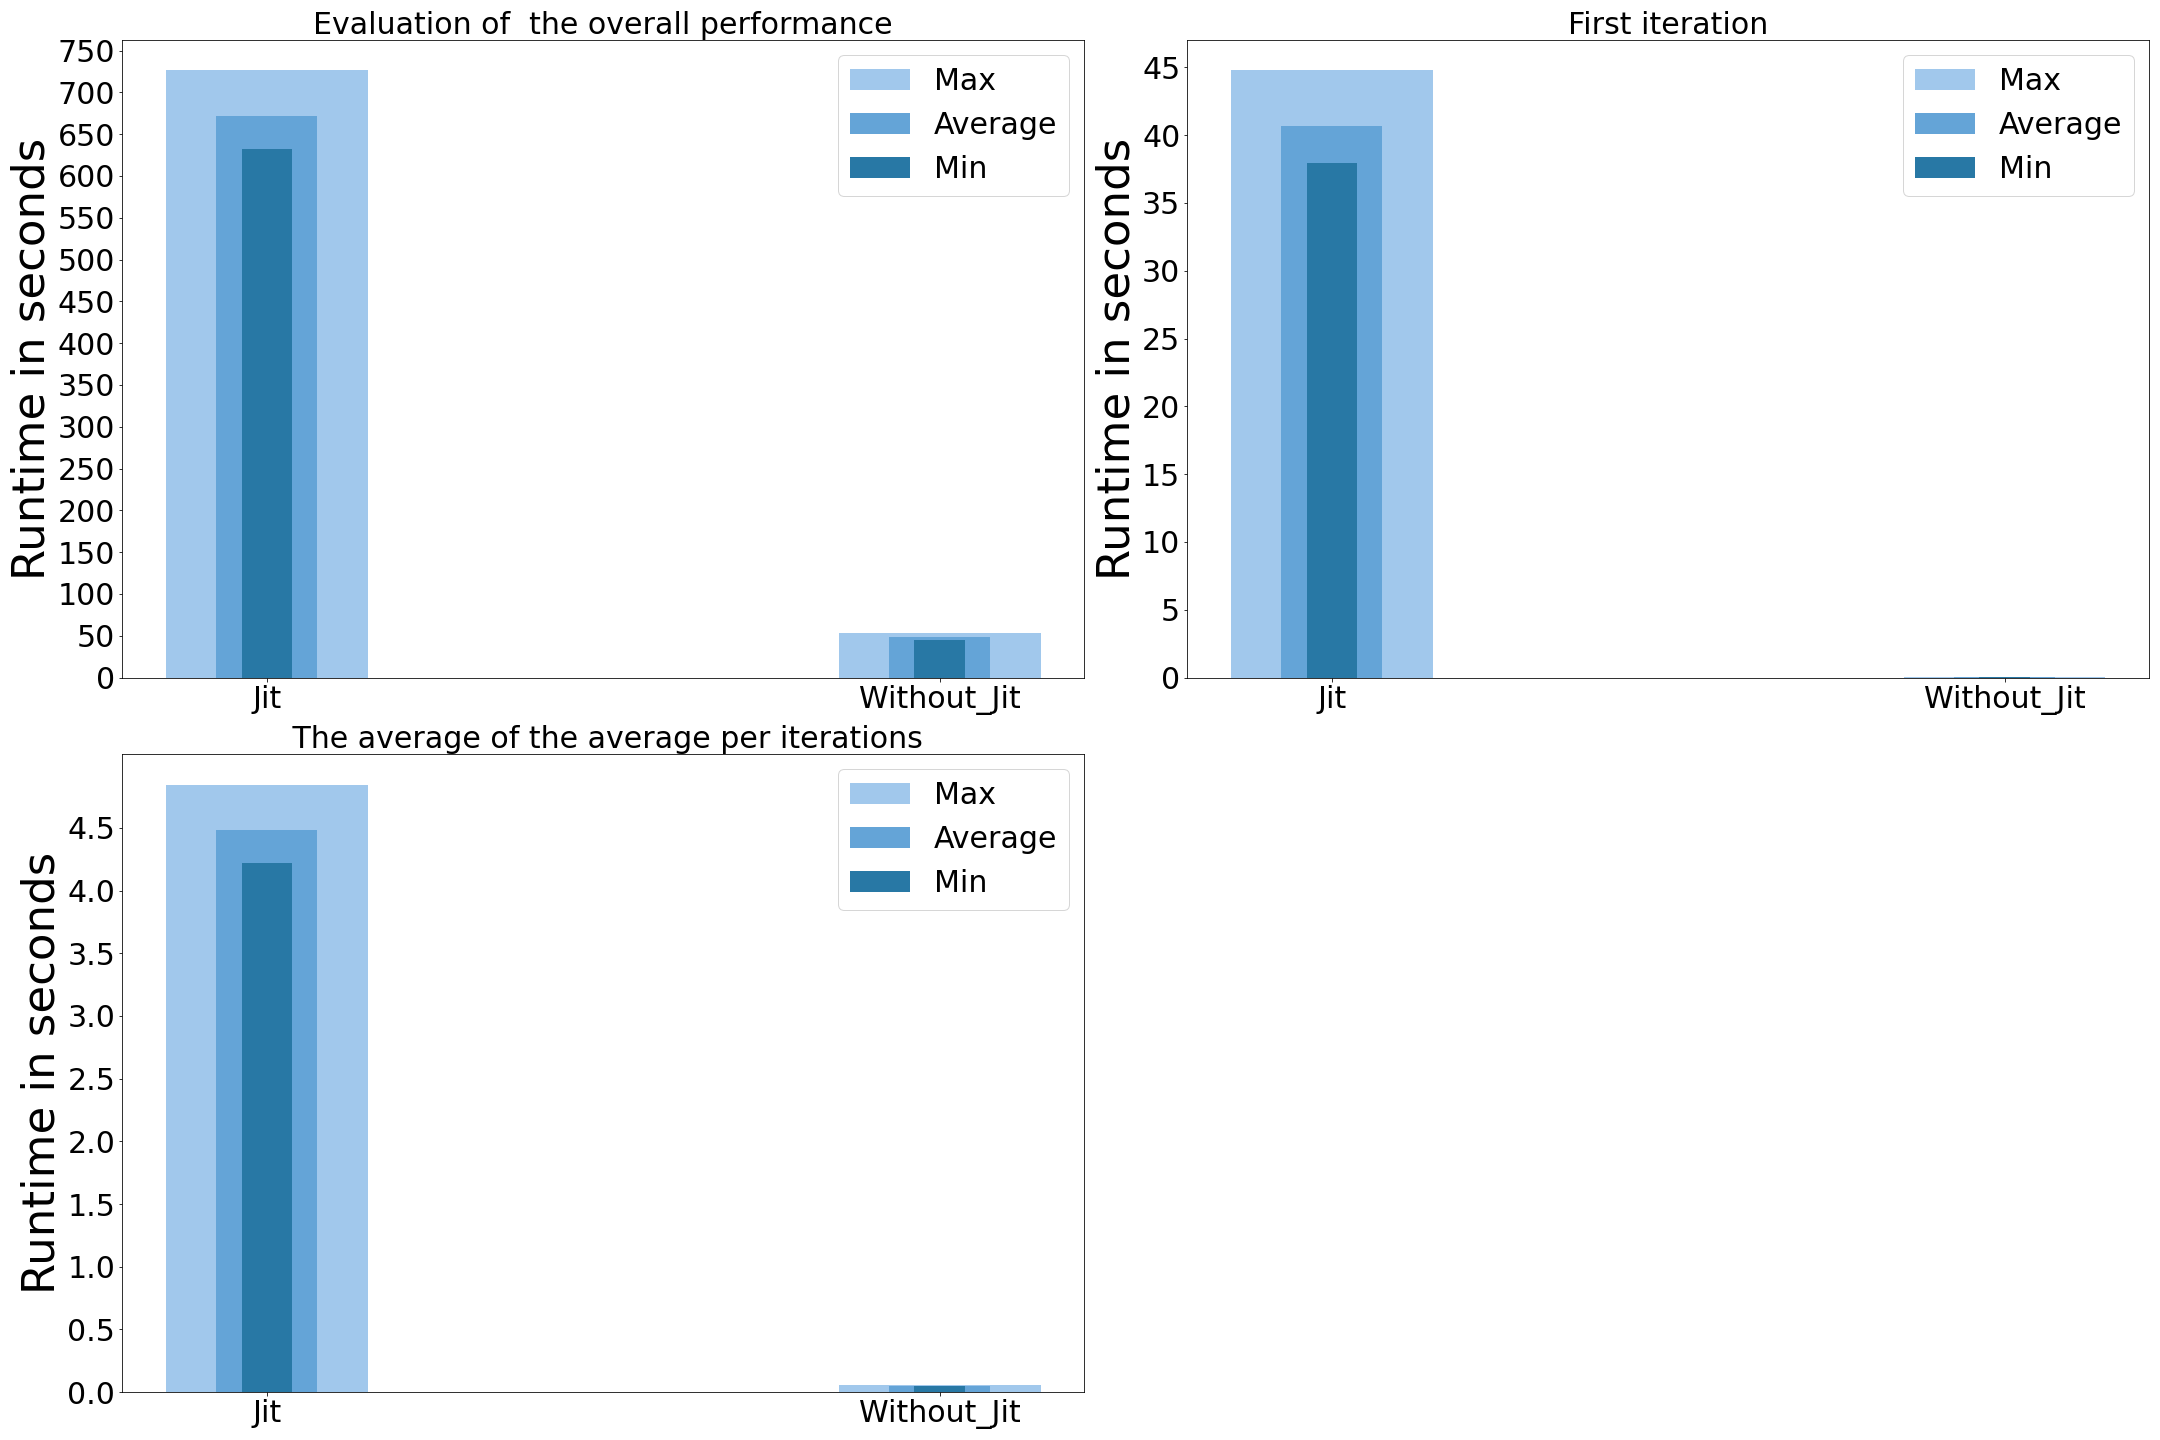
\includegraphics[width=\textwidth]{src/pic/synapse_neuron_eval.png}
    \caption{The overall runtime}
    \label{fig:overall_runtime}
\end{figure}

In the \autoref{fig:overall_runtime}, we analyze the runtime of the whole script, and then we take a look at the runtime of the function responsible for creating the network in each iteration. At the top left in the figure, we can observe the significant effect of using the \emph{JIT} module with an external synapse type.  The \emph{JIT} module requires on average more 700 seconds, whereas the normal execution took around 50 seconds to finish. The minimum runtime of the \emph{JIT} is also very high in comparison to the normal mode. If we observe the second plot at the top, we can straightforward see the reason behind the 700-second runtime. The first iteration alone took more than 40 second to finish, whereas the normal execution took less than one second to finish. This difference is caused by the same overhead discussed above, plus now we have to  trigger the code generation pipeline again and replace the \emph{source/target} elements in the network with the new correct neuron model and update its state along the synapse instance. 

In the third plot at the bottom left of the figure, we show the average time needed by all the 151 iterations in each run. As expected, the result shows that mostly only the first iteration takes the longest running time. The average is around 4.5, and it is way smaller than the average of running the first iteration. The results seem to be consistent as we have $4.5 \times 151$ is around 700 seconds. On the other hand, the average runtime of the 151 iterations without \emph{JIT} is significantly lower. As the external models will be available after the first iteration, which is the main reason why the left bottom plot shows better runtime than the first iteration, we still have the overhead of going through the \texttt{Wrapper} to execute the \emph{PyNEST} functions, which introduces a great overhead.



\section{Vectoriztation}

As \emph{NestKernel} does not completely support \emph	{vectorization} yet, we restrict our tests to the direct functions involved with the vectorized the model. We tested both the \texttt{nest.Create} and \texttt{nest.GetStatus} functions. Both experiments share the same configuration, we mainly can either change the number of created nodes and keep the number of threads constant or vice-versa. The experiments are executed with a \emph{Ryzen 7 3700u} processor with four cores and eight threads.
For the number of the nodes, we have picked \{1, 10, 30, 50,100,300,500,2000,5000,8000,1000\} and for the threads we have \{1, 2, 4, 8, 16, 32\}. Each sub-experiment is run five times, with storing the \emph{Wall} time in a \emph{csv} file containing the runtime of the \emph{vectorized} and \emph{non-vectorized} model. In each sub-experiment, we have three plots. In the first plot on the left, we show the \emph{max-average-min} runtime of the vectorized model. The middle plot shows the \emph{max-average-min} runtime of the simple \emph{non-vectorized} model. Finlay, the last plot on the most right, overlays the average runtime for both models in a single plot. The \emph{y-axis} in the first two plots shows the values after applying the \emph{logarithmic} function with base 10 on the runtime values, which were stored in microseconds, whereas the values in the last plot are only in microseconds.

\subsubsection{The Create function}

\subsubsection*{Varying the number of nodes with a constant number of threads}

 In the first configuration in testing the \texttt{nest.Create} function, we fix the number of threads and vary the number of nodes. In the  \autoref{fig:threads_1} until \autoref{fig:threads_32}, we show the results of the experiments. For each number of threads, we display the performance of the \texttt{nest.Create} function with the vectorized model against the simple models. 


In the \autoref{fig:threads_1}, we observe that both types of models behave the same until reaching a number of nodes larger than 300 ($10^{2.5}$). After that point, the vectorized model starts to become a bit slower on average, but with few microseconds. Another observation is that the \emph{min-max} area of the vectorized model is a bit fat and gets more narrow after reaching $10^3$, whereas the \emph{min-max} area is almost always narrow, and it gets more narrow after reaching 300 nodes.

In the \autoref{fig:threads_2}, we observe the same performance for both types of models, even the \emph{max-min} area looks almost the same. As in the previous experience, the performance of the vectorized model becomes a bit slower after reaching 300 nodes with a few milliseconds in comparison to the simple model. In  \autoref{fig:threads_4} with four threads, we have the same observation as in the  \autoref{fig:threads_2} with two threads.

In the rest of the figures with threads in \{8, 16, 32\}, we observe that the vectorized model gets slower and the gap between both models gets wider but still in the range of a few milliseconds.

\begin{figure}[ht!]
    \centering
    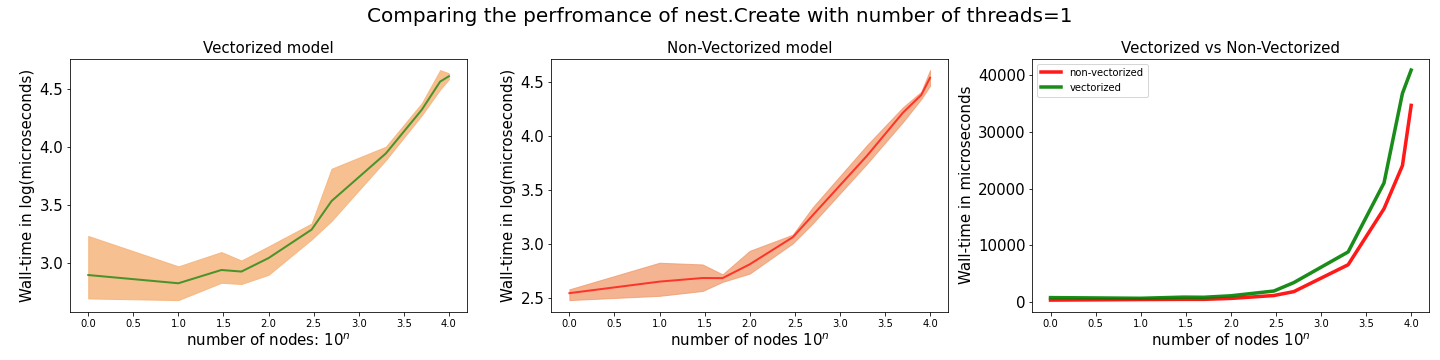
\includegraphics[width=\textwidth]{src/pic/thread_1.png}
    \caption{Performance of \texttt{nest.Create} function with the number of $threads=1$}
    \label{fig:threads_1}
\end{figure}

\begin{figure}[ht!]
    \centering
    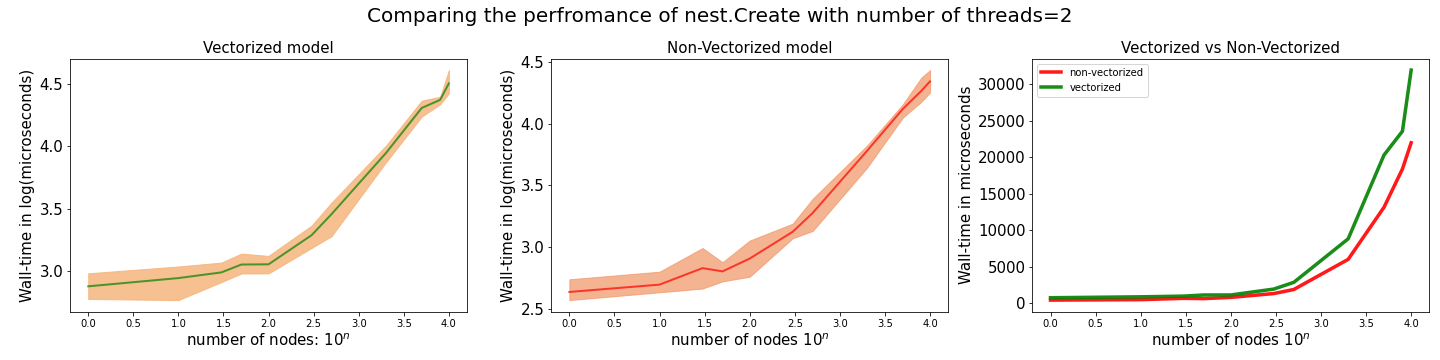
\includegraphics[width=\textwidth]{src/pic/thread_2.png}
    \caption{Performance of \texttt{nest.Create} function with the number of $threads=2$}
    \label{fig:threads_2}
\end{figure}

\begin{figure}[ht!]
    \centering
    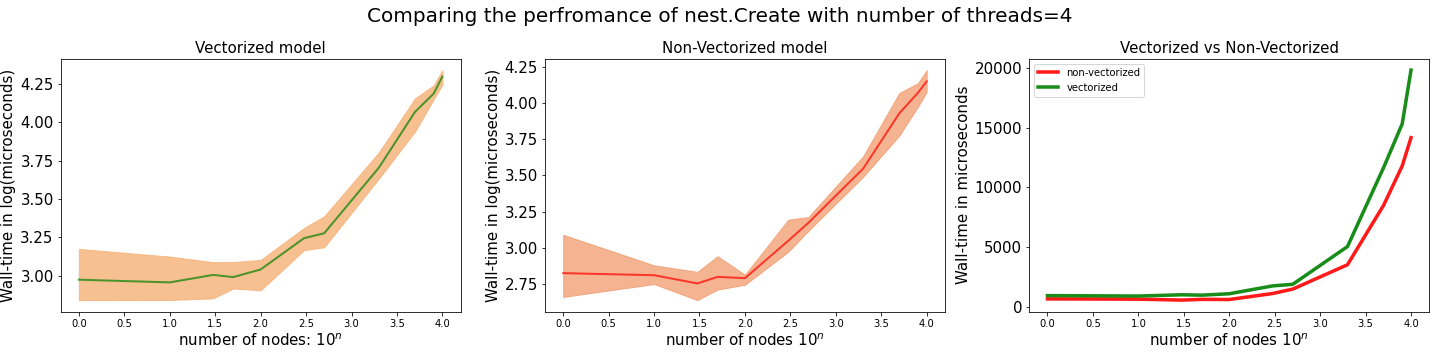
\includegraphics[width=\textwidth]{src/pic/thread_4.png}
    \caption{Performance of \texttt{nest.Create} function with the number of $threads=4$}
    \label{fig:threads_4}
\end{figure}

\begin{figure}[ht!]
    \centering
    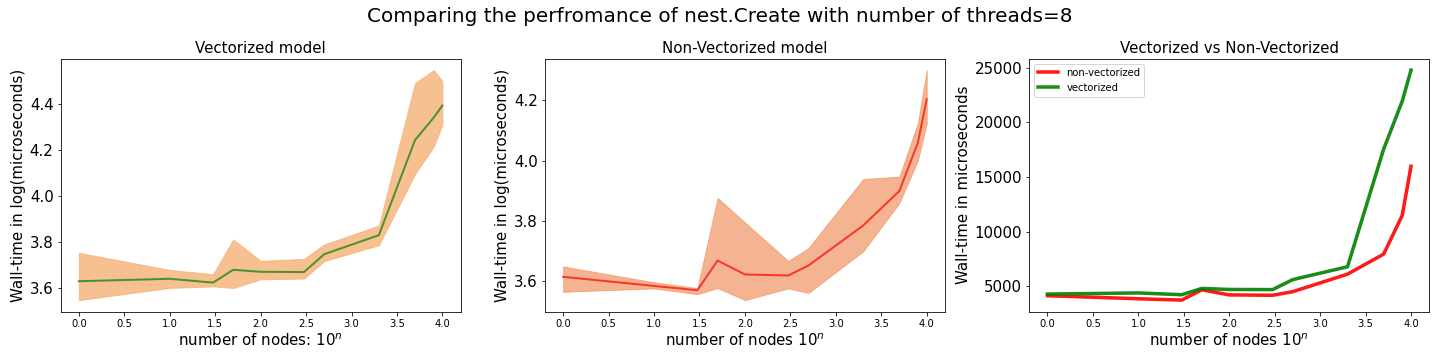
\includegraphics[width=\textwidth]{src/pic/thread_8.png}
    \caption{Performance of \texttt{nest.Create} function with the number of $threads=8$}
    \label{fig:threads_8}
\end{figure}


\begin{figure}[ht!]
    \centering
    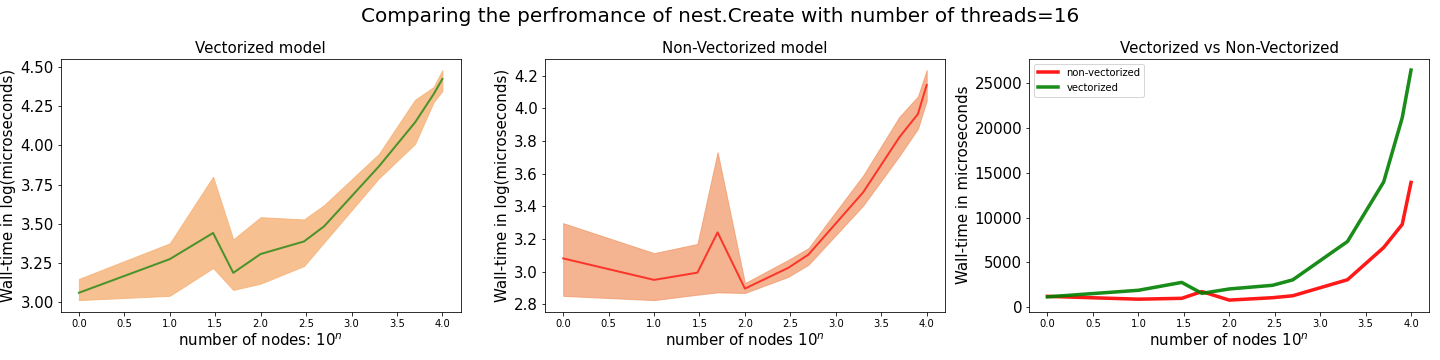
\includegraphics[width=\textwidth]{src/pic/thread_16.png}
    \caption{Performance of \texttt{nest.Create} function with the number of $threads=16$}
    \label{fig:threads_16}
\end{figure}

\begin{figure}[ht!]
    \centering
    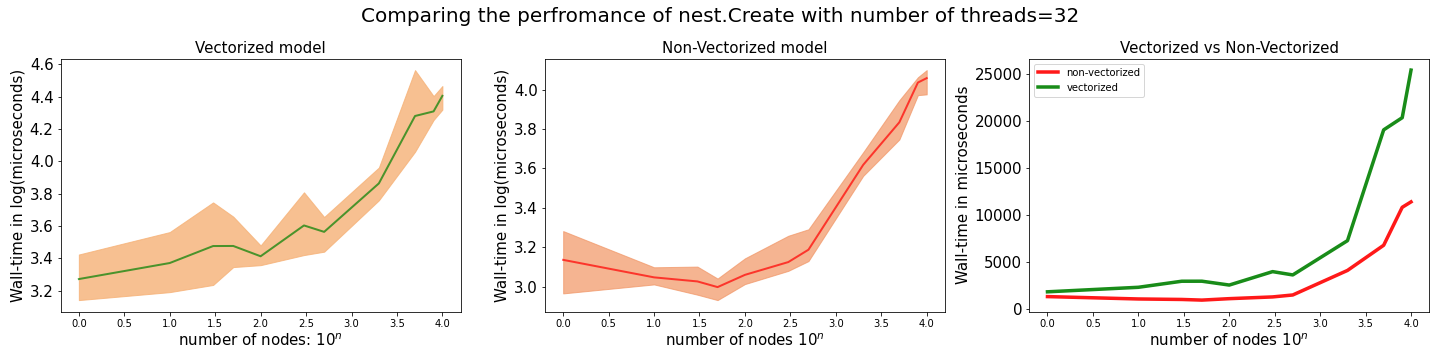
\includegraphics[width=\textwidth]{src/pic/thread_32.png}
    \caption{Performance of \texttt{nest.Create} function with the number of $threads=32$}
    \label{fig:threads_32}
\end{figure}

\subsubsection*{Varying the number of threads with a constant number of nodes}


In general, the plots between the \autoref{fig:nodes_1} and \autoref{fig:nodes_10000} show that the \texttt{nest.Create} function has a consistent behavior. In all the plots, we can observe the discontinuity that happens around the points 4, 8 and 16. At these points the slope changes significantly, and the reason behind it is the processor specification. Recall that we ran the experiments on a four-core processor. In general, the vectorized model is a bit slower than the simple model and the largest difference can be observed in the \autoref{fig:nodes_5000} with 5000 nodes. Compared to the previous experiment with fixed number of threads, the \emph{min-max} area seems to be more a bit fat, which might implicate that the current average results might be a bit noisy.

\foreach \n in {1, 10, 30, 50, 100, 300, 500, 2000, 5000, 8000, 10000}
{
\begin{figure}[ht!]
    \centering
    \includegraphics[width=\textwidth]{src/pic/nodes_\n.png}
    \caption{Performance of \texttt{nest.Create} function with the number of $nodes=$\n}
    \label{fig:nodes_\n}
\end{figure}
}

\subsubsection{The GetStatus function}

\subsubsection*{Varying the number of nodes with a constant number of threads}

Even with the \texttt{nest.GetStatus} not fully being optimized to support vectorization, both the vectorized model and the simple one has the same performance, with the vectorized model being slightly better with few microseconds.

\foreach \n in {2, 4, 8, 16, 32}
{
\begin{figure}[ht!]
    \centering
    \includegraphics[width=\textwidth]{src/pic/get_thread_\n.png}
    \caption{Performance of \texttt{nest.GetStatus} function with the number of $nodes=$\n}
    \label{fig:get_threads_\n}
\end{figure}
}

\subsubsection*{Varying the number of threads with a constant number of nodes}

The \texttt{nest.GetStatus} with varying the number of threads has a very different behavior. In the \autoref{fig:get_nodes_1}, both models have the same direction of variation with the only difference that at $threads=16$ we observe that the vectorized model is becoming a bit faster. The \emph{min-max} area in both models is also almost the same. With the number of nodes equal to ten in \autoref{fig:get_nodes_10}, we observe that between the points 6 and 16 the vectorized model is significantly faster, but then starting from 16 the vectorized model becomes slower again. In both plots, the \emph{min-max} area is very noisy.


In \autoref{fig:get_nodes_30}, both  models have the same behavior, with the vectorized model being a bit faster between the points 3 and  14 and then again after 20. Both \emph{min-max} areas have almost the same shape. In \autoref{fig:get_nodes_50}, the average performance between the models is significantly different with 1500 microseconds on average. Again, we directly observe the points where the slope of the curves changes. Those points are at position 4, 8 and 16. \autoref{fig:get_nodes_30} with 100 nodes shows also the same observations as in the \autoref{fig:get_nodes_30}.

In \autoref{fig:get_nodes_300} with 300 nodes, the vectorized model takes almost completely the lead in all thread values, with the only exception between position 6 and 10. Both \autoref{fig:get_nodes_500} and \autoref{fig:get_nodes_2000} respectively with 500 and 2000 nodes show the same observations, where the vectorized model is being faster than the simple model.

Reaching higher number of nodes as in \autoref{fig:get_nodes_5000} with 5000 nodes in \autoref{fig:get_nodes_8000} with 8000 and in \autoref{fig:get_nodes_10000} with 10000 nodes, the vectorized model is either behaving the same as the simple model or performing even better.



\foreach \n in {1, 10, 30, 50, 100, 300, 500, 2000, 5000, 8000, 10000}
{
\begin{figure}[ht!]
    \includegraphics[width=\textwidth]{src/pic/get_nodes_\n.png}
    \caption{Performance of \texttt{nest.GetStatus} function with the number of $threads=$\n}
    \label{fig:get_nodes_\n}
\end{figure}
}



\cleardoublepage
